\begin{titlepage}
\begin{tikzpicture}[remember picture,overlay,inner sep=0,outer sep=0]
     \draw[black,line width=0.5pt] ([xshift=-1.5cm,yshift=-2cm]current page.north east) coordinate (A)--([xshift= 2.5cm,yshift=-2cm]current page.north west) coordinate(B)--([xshift=2.5cm,yshift=2cm]current page.south west) coordinate (C)--([xshift=-1.5cm,yshift=2cm]current page.south east) coordinate(D)--cycle;
     
     \draw[black,line width=2pt] ([xshift=-1.6cm,yshift=-2.1cm]current page.north east) coordinate (A)--([xshift= 2.6cm,yshift=-2.1cm]current page.north west) coordinate(B)--([xshift= 2.61cm,yshift=2.1cm]current page.south west) coordinate (C)--([xshift=-1.6cm,yshift=2.1cm]current page.south east) coordinate(D)--cycle;

\end{tikzpicture}
\begin{center}
{\large Đại học Quốc gia Thành phố Hồ Chí Minh} \\[0.3em]
{\large Trường Đại học Bách Khoa} \\[0.3em]
{\large Khoa Khoa học và Kỹ thuật Máy tính} 
\end{center}

\vspace{1cm}

\begin{figure}[h!]
\begin{center}

\includegraphics[width=5cm]{img/logo/LogoBKChinhThuc.png}
\end{center}
\end{figure}

\vspace{0.5cm}


\begin{center}
\begin{tabular}{c}
\multicolumn{1}{c}{{\large LUẬN VĂN TỐT NGHIỆP ĐẠI HỌC}}

\vspace{0.5cm}
\\

\hline
\\
{\Huge Phát hiện chủ đề và phân tích xu hướng}
\\[1.5em]
\hline

\\
{\large Ngành: \space Khoa học Máy tính }


\end{tabular}
\end{center}

\vspace{1cm}

\begin{table}[h]
\begin{tabular}{rrlr}
\hspace{2.9 cm} &  GVHD: &TS. Lê Thanh Vân \\
\hspace{2.9 cm} &  GVPB: &PGS. TS. Phạm Trần Vũ\\
& SV thực hiện: &Hà Huy Long Hải         &1812064 \\

\end{tabular}
\end{table}

\vfill
\begin{center}
% {TP. Hồ Chí Minh, tháng 07 năm 2021}
{TP. Hồ Chí Minh, \today }
\end{center}
\end{titlepage}
\thispagestyle{empty}
